\documentclass[11pt]{beamer}
\title{Array Fold Logic}
\usepackage{verbatim}
\usepackage{amsmath}
\usepackage{amsthm}
\usepackage{listings}
\usepackage{graphics}
\usepackage{color}
\usepackage{stmaryrd}\usefonttheme[onlymath]{serif}

\newtheorem{proposition}{Proposition}
\author{Przemyslaw Daca et al.}
\date{\today}


\begin{document}
\maketitle
\begin{frame}\frametitle{Overview }
\begin{itemize}

\item Contributions of this paper.
\item Array fold logic: syntax, semantics and utilities.
\item Theoretical results.
\item Tool and experimental results.

\end{itemize}
\end{frame}

\begin{frame}\frametitle{Contributions}
\begin{itemize}
\item Define a new logic called AFL that can express interesting properties of counting over arrays.
\item Show the satisfiability of AFL is \textbf{PSPACE}-complete and provide a decision procedure.
\item Implement a tool \textsc{AFolder} that can solve some cases of program verification.
 
\end{itemize}
\end{frame}

\begin{frame}\frametitle{A Toy Example}
Why ``fold''? A concept in functional language which folds come function over an array.

\begin{example}
\begin{center}
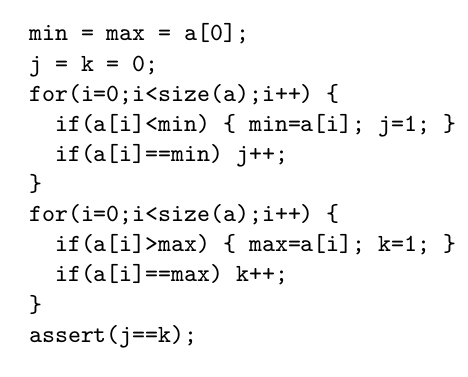
\includegraphics[scale=0.36]{c1.png}
\end{center}
\end{example}
\end{frame}

\begin{frame}\frametitle{ A Toy Example}
\begin{center}
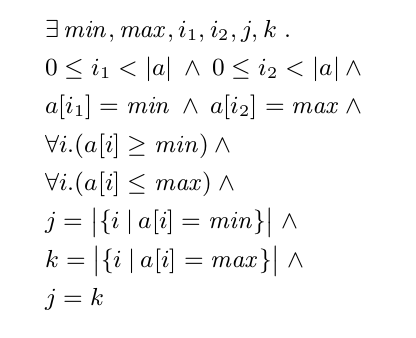
\includegraphics[scale=0.3]{f1.png}
\end{center}
This kind of formula is undecidable because we can reduce the Hilbert's 10th problem to it.
\begin{center}
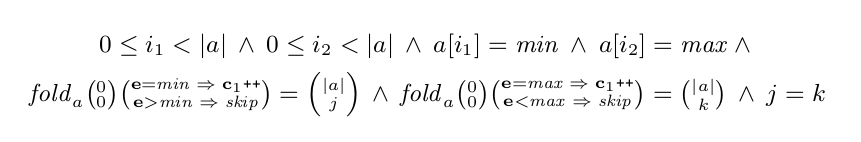
\includegraphics[scale=0.38]{afl1.png}
\end{center}
\end{frame}


\begin{frame}\frametitle{Array Fold Logic: Syntax}
\textbf{Implicit Variables:} $\{\textbf{e}, \textbf{c}_1, \ldots, \textbf{c}_{m-1}, \textbf{i}\} = FV^{m}$

\begin{itemize}
\item Array sort, \texttt{ASort}
\item Integer sort, \texttt{ISort}
\item Boolean sort, \texttt{BSort}
\item Integer vectors $\texttt{VSort}^m$
\item Functional constants $\texttt{FSort}^m = \texttt{VSort}^m\times \texttt{ISort}\rightarrow \texttt{VSort}^m$
\end{itemize}
\end{frame}

\begin{frame}\frametitle{Array Fold Logic: Syntax}

\begin{center}
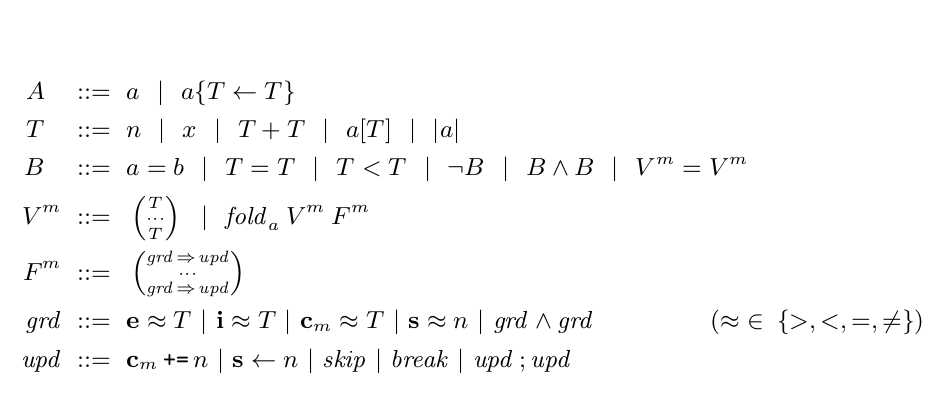
\includegraphics[scale=0.32]{aflsyn.png}
\end{center}

Given a set of function branches $Br$, we can define a control flow graph $G =\langle S,E,\gamma \rangle $.
\begin{itemize}
\item $E = \bigcup_{grd\Rightarrow upd \in Br} \{(s_1, s_2)\mid s_1 \models grd\wedge s_2 = ite(\textbf{s}\leftarrow n\in upd, n, s_1)\}$
\item $\gamma$ is the labeling of edges with the set of formulas $\Phi(grd)$ and $\Phi(upd)$.
\end{itemize}
Requirement: edges in the same SCC of $G$ update the counters in a monotonic way.

\end{frame}

\begin{frame}\frametitle{Array Fold Logic: Semantics}
$\sigma = \langle\lambda, \mu\rangle$ where $\mu: Var_{I} \rightarrow \mathbb{Z}, \lambda: Var_{A} \rightarrow \mathbb{Z}^*$.

$\kappa = FV^{m} \rightarrow \mathbb{Z}^{m+1}$
\begin{center}
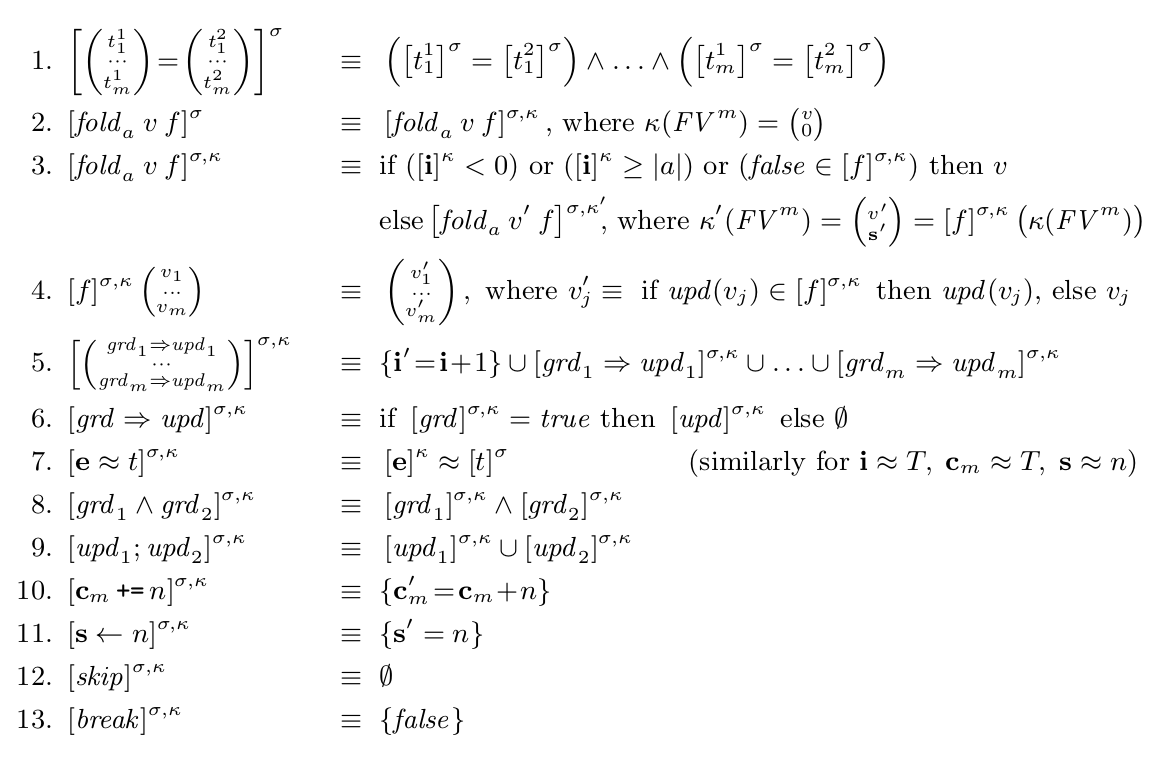
\includegraphics[scale=0.26]{aflsema.png}
\end{center}

\end{frame}


\begin{frame}\frametitle{Utility and Expressive Power}
\begin{itemize}
\item Boundedness:
\[fold_a(0)(l\le \textbf{e} \le u \Rightarrow skip) = |a|\]
\item Partitioning:
\begin{center}
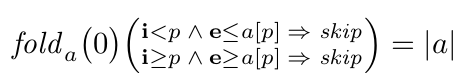
\includegraphics[scale=0.36]{partitionafl.png}
\end{center}
\item Periodic:
\begin{center}
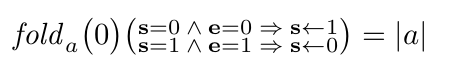
\includegraphics[scale=0.36]{periodicafl.png}
\end{center}
\item Pumping($0^n1^n$):
\begin{center}
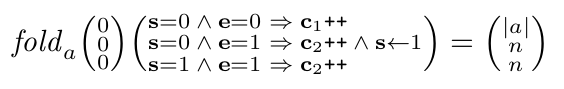
\includegraphics[scale=0.36]{pumpingafl.png}
\end{center}
\item Counting.
\end{itemize}
Properties that require universal quantification over \textit{several} index variables are inexpressive.
e.g. Sortedness and ...
\end{frame}

\begin{frame}\frametitle{Utility and Expressive Power}
\begin{itemize}
\item Loops.
\item Conditional statements.
\end{itemize}
\begin{center}
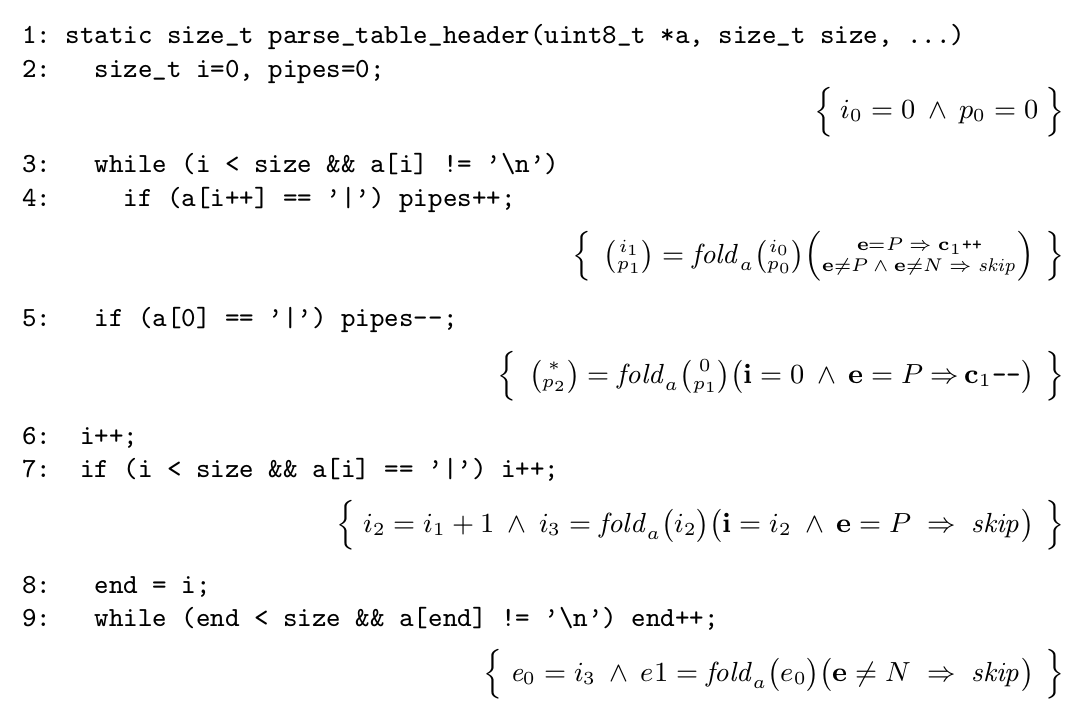
\includegraphics[scale=0.26]{mdafl.png}
\end{center}

\end{frame}

\begin{frame}\frametitle{Theoretical Results: Complexity}
\begin{definition}[symbolic $k$-counter machine]

An SMC is a tuple $\mathcal{M} = (\eta, X, Q, \delta, q^{init})$ where 
\begin{itemize}
\item $\eta$ is a vector of k counters.
\item $\delta \subseteq Q\times \texttt{CC}_k(X) \times \texttt{IC}(X)\times Q\times \mathbb{Z}^k$ is the transition relation.

\end{itemize}
\end{definition}
Translation from a functional constant $f$ of $\texttt{FSort}^m$ to an SCM.

Reversal bounded.

\[SCC_1 \rightarrow SCC_2 \rightarrow\cdots \rightarrow SCC_m\]

Parallel composition of SCMs.
\end{frame}

\begin{frame}\frametitle{Small model property}
\begin{lemma}
There exists a constant $c\in \mathbb{N}$, such that an AFL formula $\Phi$ is satisfiable iff there exists a model $\sigma$ it maps each variable in $X$ to integer that $\le 2^{|\Phi|^c}$ and array to sequence of $\le 2^{|\phi|^c}$ where each integer of the array also lies in the bound.
\end{lemma}

Give fixed counter values.

Why we want reversal-bounded?

\begin{theorem}
The satisfiability problem of AFL is \textbf{PSPACE}-complete.

\end{theorem}
Membership: NTM.

Hardness: DFA emptiness problem reduced to sat of AFL formula.

\end{frame}

\begin{frame}\frametitle{Decision Procedure}
Idea: translate the AFL formula $\phi$ into a quantifier-free PA formula $\psi = \psi_n \wedge \psi_e \wedge \psi_l$.

\begin{itemize}
\item $\psi_n$ is part of $\phi$ that does not contain fold.
\item $\psi_e$ is the reduction from the reachability problem of SMC to QFPA.
\item $\psi_l$ is the link formula used for linking some constraints between initial and final configuration in $\psi_e$.
\end{itemize}

\begin{lemma}
The complexity of satifiability of $m$-AFL for a fixed $m$ is \textbf{NP}-complete.
\end{lemma}

\end{frame}

\begin{frame}\frametitle{Experimental Results}
Tool: \textsc{AFolder} implemented on C++ and uses \textsc{Z3} for PA solving.

Benchmarks:
\begin{itemize}
\item Program RedCarpet project that is used for parsing the Markdown language.
\item NUMA(non-uniform memory access) which include multi-thread and memory operations.
\item Several cases in SV-COMP.
\item Histogram examples.
\end{itemize}
\end{frame}
\begin{frame}\frametitle{Experimental Results}
\begin{center}
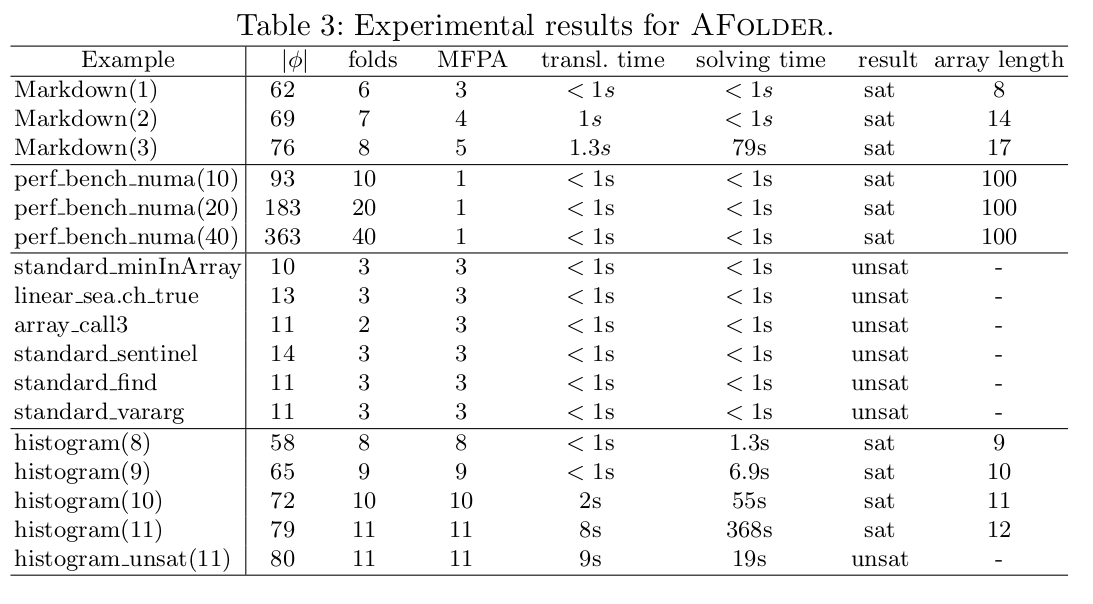
\includegraphics[scale=0.3]{expresultalf.png}
\end{center}
\end{frame}
\end{document}